\documentclass[letterpaper,9pt,twocolumn,twoside,]{pinp}

%% Some pieces required from the pandoc template
\providecommand{\tightlist}{%
  \setlength{\itemsep}{0pt}\setlength{\parskip}{0pt}}

% Use the lineno option to display guide line numbers if required.
% Note that the use of elements such as single-column equations
% may affect the guide line number alignment.

\usepackage[T1]{fontenc}
\usepackage[utf8]{inputenc}

% pinp change: the geometry package layout settings need to be set here, not in pinp.cls
\geometry{layoutsize={0.95588\paperwidth,0.98864\paperheight},%
  layouthoffset=0.02206\paperwidth, layoutvoffset=0.00568\paperheight}

\definecolor{pinpblue}{HTML}{185FAF}  % imagecolorpicker on blue for new R logo
\definecolor{pnasbluetext}{RGB}{101,0,0} %



\title{Data analysis report - Root Insurance}

\author[a]{Issac Lee}

  \affil[a]{Department of Statistics \& Actuarial Science, 241 Schaeffer Hall, Iowa
City, Iowa 52242-1409}

\setcounter{secnumdepth}{0}

% Please give the surname of the lead author for the running footer
\leadauthor{Author and Author}

% Keywords are not mandatory, but authors are strongly encouraged to provide them. If provided, please include two to five keywords, separated by the pipe symbol, e.g:
 

\begin{abstract}
This report illustrates how I approach the project and the decision
making the process for Root insurance's data analysis project. The goal
of this project is to find the best-matched OBDII trip data, which
corresponds to a trip data from a user's smartphone. The data analysis
process appears in the first chapter, and the instructional manual
follows in the later chapter. The \texttt{R} code implementations follow
Google's \texttt{R} code style guide.
\end{abstract}

\dates{This version was compiled on \today} 

% initially we use doi so keep for backwards compatibility
% new name is doi_footer
\doifooter{\url{https://cran.r-project.org/package=YourPackage}}

\pinpfootercontents{YourPackage Vignette}

\begin{document}

% Optional adjustment to line up main text (after abstract) of first page with line numbers, when using both lineno and twocolumn options.
% You should only change this length when you've finalised the article contents.
\verticaladjustment{-2pt}

\maketitle
\thispagestyle{firststyle}
\ifthenelse{\boolean{shortarticle}}{\ifthenelse{\boolean{singlecolumn}}{\abscontentformatted}{\abscontent}}{}

% If your first paragraph (i.e. with the \dropcap) contains a list environment (quote, quotation, theorem, definition, enumerate, itemize...), the line after the list may have some extra indentation. If this is the case, add \parshape=0 to the end of the list environment.


\hypertarget{data-preparation}{%
\subsection{Data Preparation}\label{data-preparation}}

There are two telematics data set from independent sensors: GPS in
smartphone, OBDII. The two data sets are provided as two separate file.
Here we assume that the two \texttt{json} files are extracted in the
working directory, which means you have the following two files in the
working directory:

\begin{quote}
mobile\_trips.json, obd2\_trips.json
\end{quote}

\hypertarget{data-load-and-structure}{%
\subsection{Data load and structure}\label{data-load-and-structure}}

Since the two files are recorded as \texttt{json} format,
\texttt{jsonlite} package will be used to load the data.

\begin{Shaded}
\begin{Highlighting}[]
\KeywordTok{library}\NormalTok{(jsonlite)}

\CommentTok{# read mobile trip & obd2 trip}
\NormalTok{mobile_data <-}\StringTok{ }\KeywordTok{fromJSON}\NormalTok{(}\StringTok{"./mobile_trips.json"}\NormalTok{)}
\NormalTok{obd2_data <-}\StringTok{ }\KeywordTok{fromJSON}\NormalTok{(}\StringTok{"./obd2_trips.json"}\NormalTok{)}
\end{Highlighting}
\end{Shaded}

Smartphone data set consisists of 44 trips and OBDII data set consists
of 41 trips. The colum names of the each data set and the data types are
as follows:

\begin{itemize}
\tightlist
\item
  OBDII data

  \begin{itemize}
  \tightlist
  \item
    trip\_id (\texttt{char}), timestamp (\texttt{dbl}), speed
    (\texttt{int})
  \end{itemize}
\item
  Mobile data

  \begin{itemize}
  \tightlist
  \item
    trip\_id (\texttt{char}), created\_at (\texttt{dbl}), timestamp
    (\texttt{dbl}), speed (\texttt{dbl}), accuracy (\texttt{int})
  \end{itemize}
\end{itemize}

\hypertarget{visualization-of-sample-trips}{%
\subsection{Visualization of sample
trips}\label{visualization-of-sample-trips}}

Fig \ref{fig:rawplot_obd2} shows the sample speed graph of one of the
trips from OBDII data. As we can see, the trip was recorded for around
1,200 seconds and we do not know the unit for the recorded speed. By
examing the data set littel bit, it can be easily realized that the
first trip from each sources corresponds to each other as in Fig.
\ref{fig:rawplot_obd2} and Fig \ref{fig:rawplot_mobile}.

\begin{figure}

{\centering 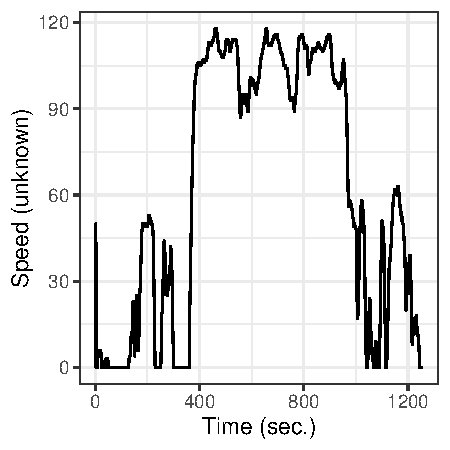
\includegraphics{report_issaclee_files/figure-latex/rawplot_obd2-1} 

}

\caption{A sample of speed graph of OBDII (the 1st trip).}\label{fig:rawplot_obd2}
\end{figure}

\begin{figure}

{\centering 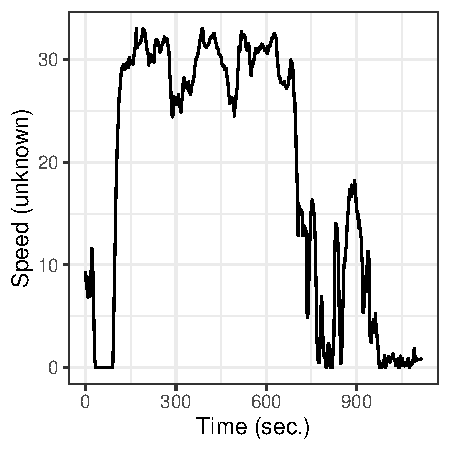
\includegraphics{report_issaclee_files/figure-latex/rawplot_mobile-1} 

}

\caption{A sample of speed graph of Smartphone (the 1st trip).}\label{fig:rawplot_mobile}
\end{figure}

This \emph{pinp is not PNAS} template started when the introduction to
\href{http://dirk.eddelbuettel.com/code/rcpp.html}{Rcpp} by
\cite{PeerJ:Rcpp} was converted into this updated
\href{https://eddelbuettel.github.io/pinp/Rcpp-introduction.pdf}{Rcpp
Introduction} vignette. It is based on the
\href{https://github.com/rstudio/rticles/tree/master/inst/rmarkdown/templates/pnas_article}{pnas\_article}
template of the wonderful
\href{https://cran.r-project.org/package=rticles}{rticles} package by
\cite{CRAN:rticles}. The conversion from markdown to latex is
facilitated by
\href{https://cran.r-project.org/package=rmarkdown}{rmarkdown}
\citep{CRAN:rmarkdown} and
\href{https://cran.r-project.org/package=knitr}{knitr}
\citep{CRAN:knitr}. The underlying LaTeX macros are from
\href{http://www.pnas.org/site/authors/latex.xhtml}{pnas.org}.

The remainder of the document carries over from the corresponding
\href{https://github.com/rstudio/rticles/tree/master/inst/rmarkdown/templates/pnas_article}{pnas\_article}
template document. but has been edited and updated to our use case. A
few specific tips follow. In general, for fine-tuning some knowledge of
LaTeX is helpful.

\hypertarget{author-affiliations}{%
\subsection{Author Affiliations}\label{author-affiliations}}

Per common academic best practice, you can include your department,
institution, and complete address, with the ZIP/postal code, for each
author. Use lower case letters to match authors with institutions, as
shown in the example. Authors with an ORCID ID may supply this
information at submission.

\hypertarget{document-options}{%
\subsection{Document Options}\label{document-options}}

We support several options via the YAML header

\begin{itemize}
\tightlist
\item
  Setting a DOI or URL footer, for example for the CRAN package URL,
  which is placed in the bottom-left footer of the title page and even
  pages;
\item
  Setting a footer label, for example \emph{YourPackage Vignette}
  stating your package, which is placed in the bottom-right footer on
  odd pages;
\item
  Setting a free-form author field used on the inside footer;
\item
  Optional \emph{Draft} watermark to be added to each page;
\item
  Line of custom text in subtitle (\texttt{date\_subtitle}) suitable to
  give publication info of the draft, e.g.~journal name in a post-print.
\end{itemize}

\hypertarget{references}{%
\subsection{References}\label{references}}

Here we differ from PNAS and suggest natbib. References will appear in
author-year form. Use \texttt{\textbackslash{}citet\{\}},
\texttt{\textbackslash{}citep\{\}}, etc as usual.

We default to the \texttt{jss.bst} style. To switch to a different
bibliography style, please use \texttt{biblio-style:\ style} in the YAML
header.

\hypertarget{inline-r-code}{%
\subsection{Inline R Code}\label{inline-r-code}}

The PNAS sample included a fixed PNG image here, but this document
prefers to show the results and embedding of \emph{R} code.

\begin{Shaded}
\begin{Highlighting}[]
\KeywordTok{library}\NormalTok{(ggplot2)}
\KeywordTok{ggplot}\NormalTok{(mtcars, }\KeywordTok{aes}\NormalTok{(wt, mpg)) }\OperatorTok{+}
\StringTok{    }\KeywordTok{geom_point}\NormalTok{(}\DataTypeTok{size=}\DecValTok{3}\NormalTok{, }\KeywordTok{aes}\NormalTok{(}\DataTypeTok{colour=}\KeywordTok{factor}\NormalTok{(cyl))) }\OperatorTok{+}
\StringTok{    }\KeywordTok{theme}\NormalTok{(}\DataTypeTok{legend.position=}\StringTok{"none"}\NormalTok{)}
\end{Highlighting}
\end{Shaded}

\begin{figure}

{\centering 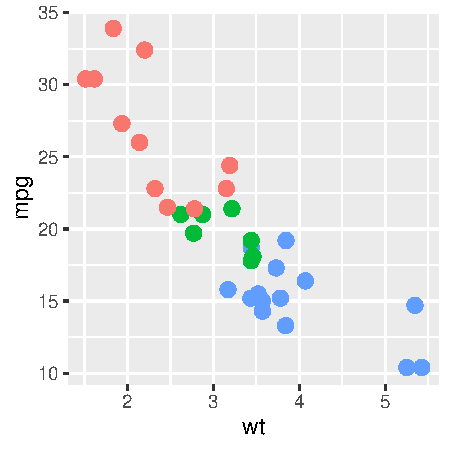
\includegraphics{report_issaclee_files/figure-latex/figex-1} 

}

\caption{Narrow ggplot2 figure}\label{fig:figex}
\end{figure}

Here we use a standard knitr bloc with explicit options for

\begin{itemize}
\tightlist
\item
  figure width and height (\texttt{fig.width}, \texttt{fig.height}),
  both set to three inches;
\item
  whether the code is shown (\texttt{echo=TRUE}); and
\item
  the caption (\texttt{fig.cap}) as shown above.
\end{itemize}

\hypertarget{digital-figures}{%
\subsection{Digital Figures}\label{digital-figures}}

Markdown, Pandoc and LaTeX support \texttt{.eps} and \texttt{.pdf}
files.

Figures and Tables should be labelled and referenced in the standard way
using the \texttt{\textbackslash{}label\{\}} and
\texttt{\textbackslash{}ref\{\}} commands.

The R examples above show how to insert a column-wide figure. To insert
a figure wider than one column, please use the
\texttt{\textbackslash{}begin\{figure*\}...\textbackslash{}end\{figure*\}}
environment.

One (roundabout) way of doing this is to \emph{not} actually plot a
figure, but to save it in a file as the following segment shows:

\begin{Shaded}
\begin{Highlighting}[]
\KeywordTok{library}\NormalTok{(ggplot2)}
\NormalTok{p <-}\StringTok{ }\KeywordTok{ggplot}\NormalTok{(}\DataTypeTok{data =}\NormalTok{ midwest,}
            \DataTypeTok{mapping =} \KeywordTok{aes}\NormalTok{(}\DataTypeTok{x =}\NormalTok{ area,}
                          \DataTypeTok{fill =}\NormalTok{ state,}
                          \DataTypeTok{color =}\NormalTok{ state)) }\OperatorTok{+}
\StringTok{    }\KeywordTok{geom_density}\NormalTok{(}\DataTypeTok{alpha =} \FloatTok{0.3}\NormalTok{)}
\CommentTok{## save to file}
\KeywordTok{suppressMessages}\NormalTok{(}\KeywordTok{ggsave}\NormalTok{(}\StringTok{"densities.pdf"}\NormalTok{, p))}
\end{Highlighting}
\end{Shaded}

This file is then included via standard LaTeX commands.

\begin{figure*}
  \begin{center}
    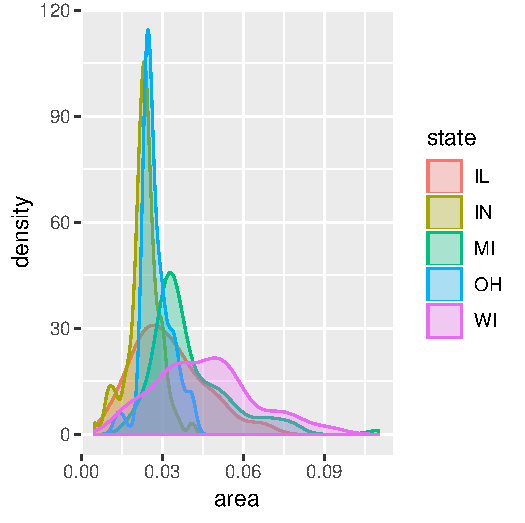
\includegraphics[width=0.66\textwidth, height=3.5in]{densities} 
  \end{center}
  \caption{Wide ggplot2 figure}\label{fig}
\end{figure*}

\hypertarget{typeset-code-but-do-not-run-it}{%
\subsection{Typeset Code (But Do Not Run
It)}\label{typeset-code-but-do-not-run-it}}

We can also just show code.

\begin{Shaded}
\begin{Highlighting}[]
\NormalTok{xx <-}\StringTok{ }\NormalTok{faithful[,}\StringTok{"eruptions"}\NormalTok{]}
\NormalTok{fit <-}\StringTok{ }\KeywordTok{density}\NormalTok{(xx)}
\KeywordTok{plot}\NormalTok{(fit)}
\end{Highlighting}
\end{Shaded}

This simply used a pandoc bloc started and ended by three backticks,
with \texttt{r} as the language choice. Similarly, \emph{many} other
languages can be typeset directly simply by relying on pandoc.

\hypertarget{single-column-equations}{%
\subsection{Single column equations}\label{single-column-equations}}

Authors may use 1- or 2-column equations in their article, according to
their preference.

To allow an equation to span both columns, options are to use the
\texttt{\textbackslash{}begin\{figure*\}...\textbackslash{}end\{figure*\}}
environment mentioned above for figures. The
\texttt{\textbackslash{}begin\{widetext\}...\textbackslash{}end\{widetext\}}
environment as shown in equation \ref{eqn:example} below is deprecated,
but \LaTeX commands \texttt{\textbackslash{}onecolumn} and
\texttt{\textbackslash{}twocolumn} work fine.

Please note that this option may run into problems with floats and
footnotes, as mentioned in the \href{http://texdoc.net/pkg/cuted}{cuted
package documentation}. In the case of problems with footnotes, it may
be possible to correct the situation using commands
\texttt{\textbackslash{}footnotemark} and
\texttt{\textbackslash{}footnotetext}.

\begin{equation}
  \begin{aligned}
(x+y)^3&=(x+y)(x+y)^2\\
       &=(x+y)(x^2+2xy+y^2) \\
       &=x^3+3x^2y+3xy^3+x^3. 
       \label{eqn:example} 
  \end{aligned}
\end{equation}

%\showmatmethods


\bibliography{pinp.bib}
\bibliographystyle{jss}



\end{document}

